\newcommand{\duedate}{26 September 2024}
\documentclass{16384_doc} %% Change for your computer

\newcommand{\assignmentname}{Assignment 3: Inverse Differential Kinematics}

\begin{document}
\maketitle

\tableofcontents

\section{Overview}
This assignment reinforces the following topics:
\begin{itemize}

\item Jacobians
\item Psuedoinverses

\end{itemize}

\section{Background}

\subsection{The Inverse Problem}
So far we have studied the functions that perform forward kinematics, which
means going from a manipulator's configuration space, $Q$ to its workspace, $W$:

\[
W = f(Q)
\]

\noindent In other words, we have determined the function for a robot arm that uses its
joint angles to calculate the position and orientation of its end effector (as
well as other frames on the robot).

You can probably think of a lot of cases where we want to do the inverse: given
a specified effector position (and potentially orientation), what are the joint
angles that will achieve this?  This inverse process is problematic because the
forward kinematics function, $f$, is (usually) non-linear.  That means that we
(usually) cannot just say:

\[
Q = f^{-1}(W)
\]

This means that finding the inverse function for the kinematics of an arm is
difficult (but by no means impossible---in the next assignment we will
tackle several methods to do this).

\subsection{Differential IK}
While the general problem of going from workspace positions to joint angles is
difficult, we can begin with the \emph{differential} problem -- going from
workspace velocities to configuration space velocities.
\[
\dot q = f^{-1}(\dot w)
\]

From the last assignment, you know that the function relating these two sets
of velocities is the Jacobian, $J$.  A key property of the Jacobian is that it is
linear (given the configuration $q$ of the arm).  In practical terms, this means
that if we know an arm’s joint angles and desired instantaneous end-effector
velocities, we can calculate the required joint velocities by inverting the
Jacobian:
\[
\dot q = J^{-1}(q) \dot w
\]

Because (for a given configuration) the Jacobian can be represented as a matrix, this is a much easier problem than the general IK problem we began with. It doesn't directly give us
the joint angles for a given end effector position, but it can be used to help
solve for these, as we'll see in the assignment.

\subsection{Pseudoinverse}

But wait---although inverting matrices is easy for computers, not all matrices
(and not all Jacobians) are invertible!  In order for a matrix to be invertible,
it has to be square, and have a non-zero determinant.  In terms of a robot arm
this means that it has to be:
\begin{itemize}
 \item Fully constrained (the same number of workspace and configuration space
  variables)
 \item Non-singular (the arm’s instantaneous motion can span the dimension of
  the workspace, meaning $J$ is full rank)
\end{itemize}

Fortunately, mathematicians have developed a technique called the
\emph{pseudoinverse} to help get around the problem of not having a square or
full rank matrix.  The pseudoinverse has some, but not all, of the properties of
a true matrix inverse.  The general method to compute this quantity involves
a technique called \emph{singular value decomposition}, but when the matrix is
\emph{full rank}, there are analytical formulas that can be used to find the inverse.

In this case, we basically make the matrix square by multiplying it by its
transpose.  We then invert the new matrix, and multiply the result by the
transpose of the original matrix to get the dimensions to match up. The exact
order of multiplication depends on the dimension of the matrix:

\subsubsection{Underconstrained}
To determine the joint velocities that result in a given a workspace velocity, we need to solve a system of linear equations (given a joint configuration).   If there are $n$ joint variables and $m$ workspace variables, then the Jacobian has dimensions $m \times n$.  Consider the case where $m < n$ i.e. there are more joints than the number of workspace variables. This results in a system of m equations (i.e. constraints) in n unknowns (i.e. joint velocities) where $m < n$, hence the name underconstrained.

Assuming the Jacobian is full rank, such a system always has a solution. This means we can always find joint velocities that result in a given end effector velocity. However, there is a whole family of solutions that satisfy these constraints. Therefore, one might be interested in searching the best solution in this family, measured with respect to some criterion. For the purpose of this discussion, we are interested in solutions (joint velocities) which result in the smallest effort in moving the arm. We can quantify this effort using the squared norm of the joint velocities.

Posing this as an optimization problem, we want to find $\dot q$ such that we minimize $\dot q^T \dot q$ satisfying $\dot w = J(q) \dot q$, where $\dot w$ and $J(q)$ are known.

This optimization problem is equivalent to a least-norm problem for linear systems of equations and has an exact analytical solution given by:
\[
\dot q = J^+ \dot w,
\]
% \begin{equation}
% \Qd = J^+\Wd
% \end{equation}
where $J^+$ is known as the right pseudoinverse of the Jacobian and is given by:
\[
J^+ = J^T(JJ^T)^{-1}
\]
% \begin{equation*}
% J^{+} = J^T(JJ^T)^{-1}
% \end{equation*}


\subsubsection{Overconstrained}
This case is when the number of rows the Jacobian has is greater than (or equal
to) the number of columns. In other words, there are more equations than unknowns.

In this case, the arm cannot move the end effector with the exact desired
velocity, but this solution will try to solve for the ``best'' joint velocities in
terms of the sum-squared error of end effector velocities. This is called the left puesdoinverse.
% \begin{equation*}
% J^{\#} = (J^TJ)^{-1}J^T
% \end{equation*}
\[
J^\# = (J^TJ)^{-1}J^T
\]

As a side note, the pseudoinverse in this overconstrained case is really useful
even outside of kinematics, and is used to quickly and reliably do things like
solve for best-fit lines to data.

\subsubsection{Perfectly Constrained}
Note that in the case of a square full rank matrix, the psuedoinverse will
result in $J^{-1}$.

\subsection{Course Logistics}

In this class you would be using the following websites regularly:
\begin{itemize}
    \item \href{https://canvas.cmu.edu/courses/42018}{Canvas}: The main course web page. This links to everything relevant to the class (including the next two links).
    \item \href{https://piazza.com/class/m09xl90abke42b}{Piazza}: This is the best way to ask course staff questions, and see course announcements.
    \item \href{https://www.gradescope.com/courses/820155/assignments/4876306/submissions}{Gradescope}: This is where you will be turning in your homework. You should have already been added to the course. If you haven't, please contact the course staff via email or Piazza post.
\end{itemize}    

\writtenSection

\section{Written Questions}
% For all of the following questions, please fully compute all answers and show
% your work for full credit, unless otherwise specified. Submit your answers in a
% PDF entitled \verb!writeup.pdf! in your handin directory.  All answers must be
% typed, but diagrams may be hand-drawn and scanned in.  However, they must be
% tidy and fully legible! Consider drawing them in a black or blue pen.  All units
% are in radians and meters, where appropriate.

\begin{questions}

    \titledquestion{R Robot}
    Consider the following robot
    \begin{center}
    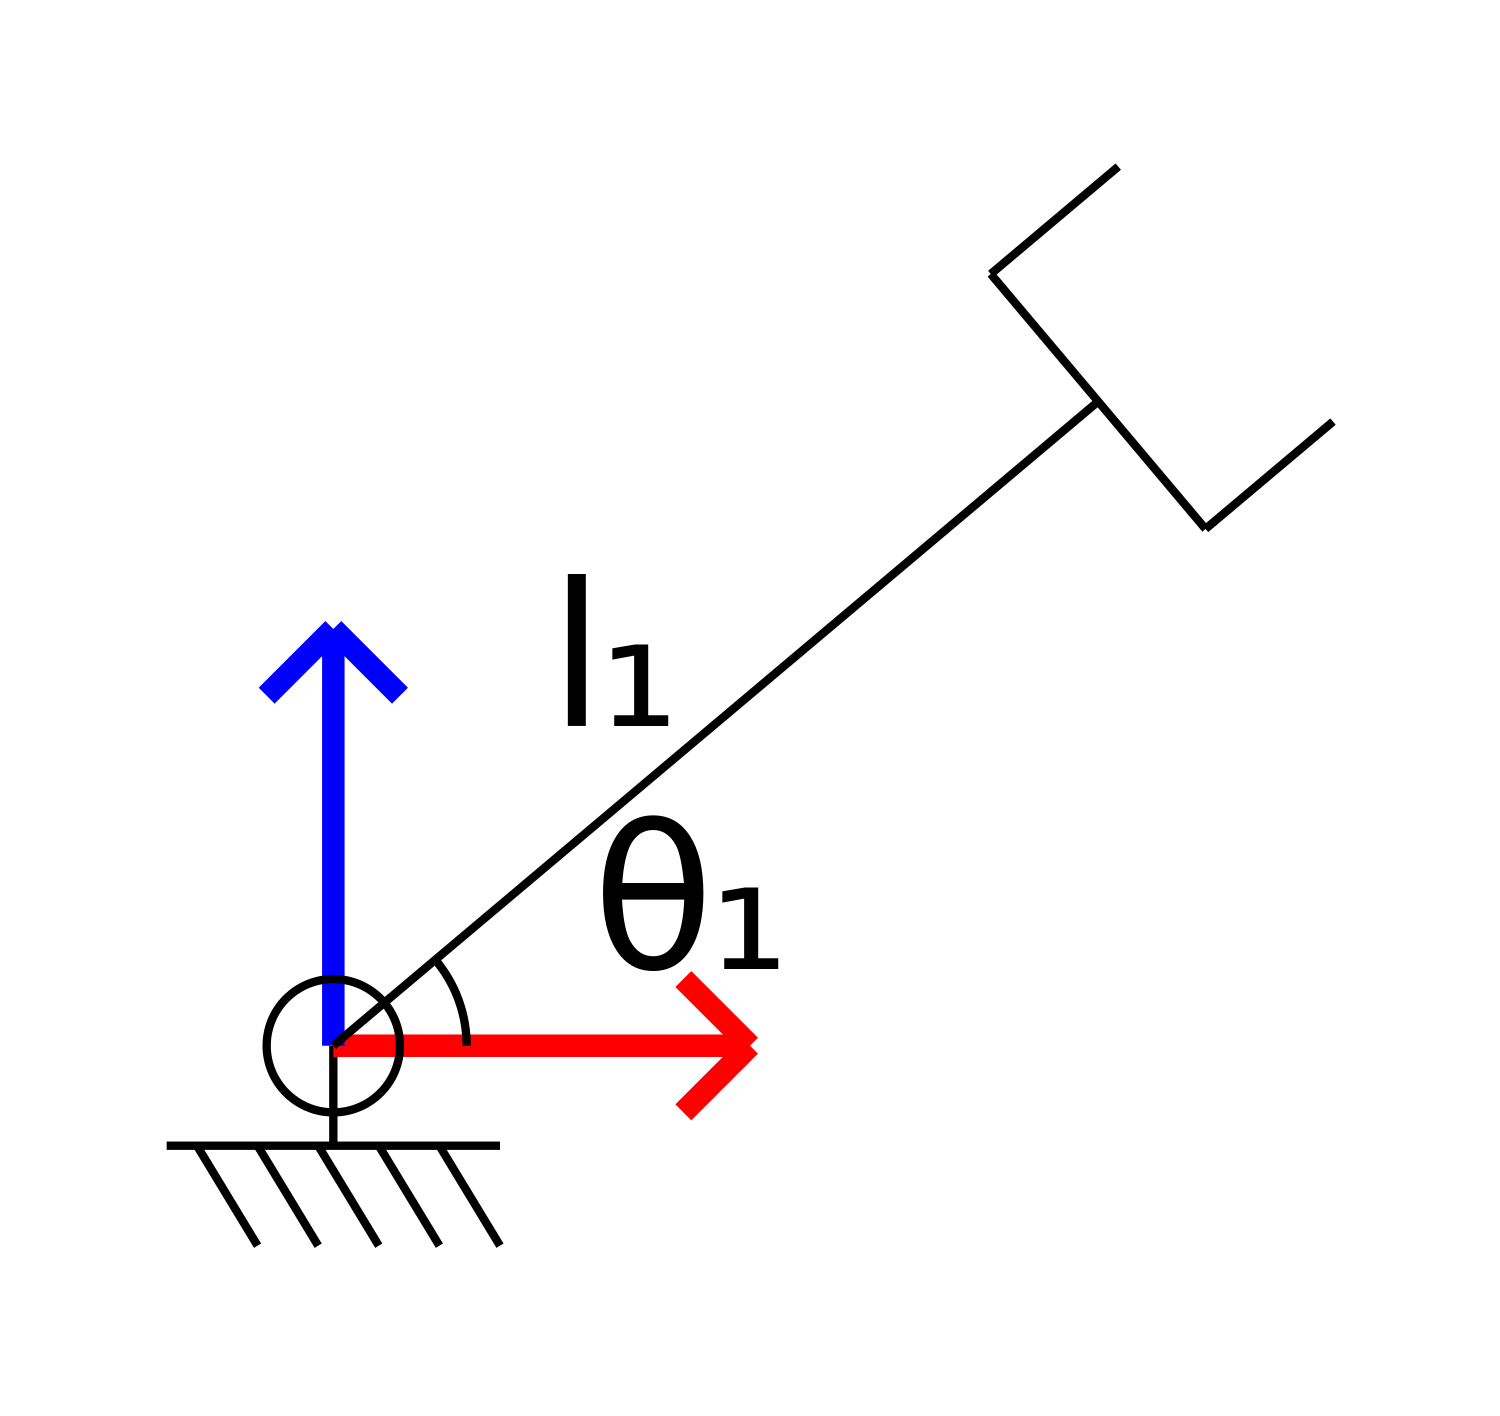
\includegraphics[scale=0.07]{generated_figures/R_nonsingular.png}
    \end{center}

        Assume \th[1] = \piover{4}.
    \begin{enumerate} [label=\alph*.]
        \item \text{[1 point]} What is the dimension of the end-effector Jacobian? Consider
        end-effector positions $\begin{bmatrix} x\\ y \end{bmatrix}$ in $\mathbb{R}^2$.
        \begin{tcolorbox}[height=3cm]
            % TODO: ENTER YOUR ANSWER HERE
        \end{tcolorbox}
        
        \item \text{[1 point]} Is this system underconstrained, overconstrained, or neither?
        Why?
        \begin{tcolorbox}[height=3cm]
            % TODO: ENTER YOUR ANSWER HERE
        \end{tcolorbox}

        
        \item \text{[2 points]} Draw the velocity vector for the end effector caused by joint 1
        moving with unit velocity. The direction of these vectors should be
        correct, but do not worry about the magnitude. You can complete this
        problem by inspection or by using properties of the Jacobian.

        \begin{tcolorbox}[height=3cm]
            % TODO: ENTER YOUR ANSWER HERE
        \end{tcolorbox}
        
        \item \text{[2 points]} What is the dimension of the space spanned by this vector?
        \begin{tcolorbox}[height=3cm]
            % TODO: ENTER YOUR ANSWER HERE
        \end{tcolorbox}
        
        \item \text{[1 point]} What is the rank of $J$ for this configuration?
        \begin{tcolorbox}[height=3cm]
            % TODO: ENTER YOUR ANSWER HERE
        \end{tcolorbox}
        
        \item \text{[1 point]} When identifying the inverse differential kinematics for this
        problem, would you use the inverse, the left psuedoinverse, or the right
        psuedoinverse?
        \begin{tcolorbox}[height=3cm]
            % TODO: ENTER YOUR ANSWER HERE
        \end{tcolorbox}
        
        \item \text{[3 points]} What are the benefits of a left pseudoinverse versus a right
        pseudoinverse?
        \begin{tcolorbox}[height=3cm]
            % TODO: ENTER YOUR ANSWER HERE
        \end{tcolorbox}
        
    \end{enumerate}

    \titledquestion{RR Robot}
    Consider the following robot
    \begin{center}
    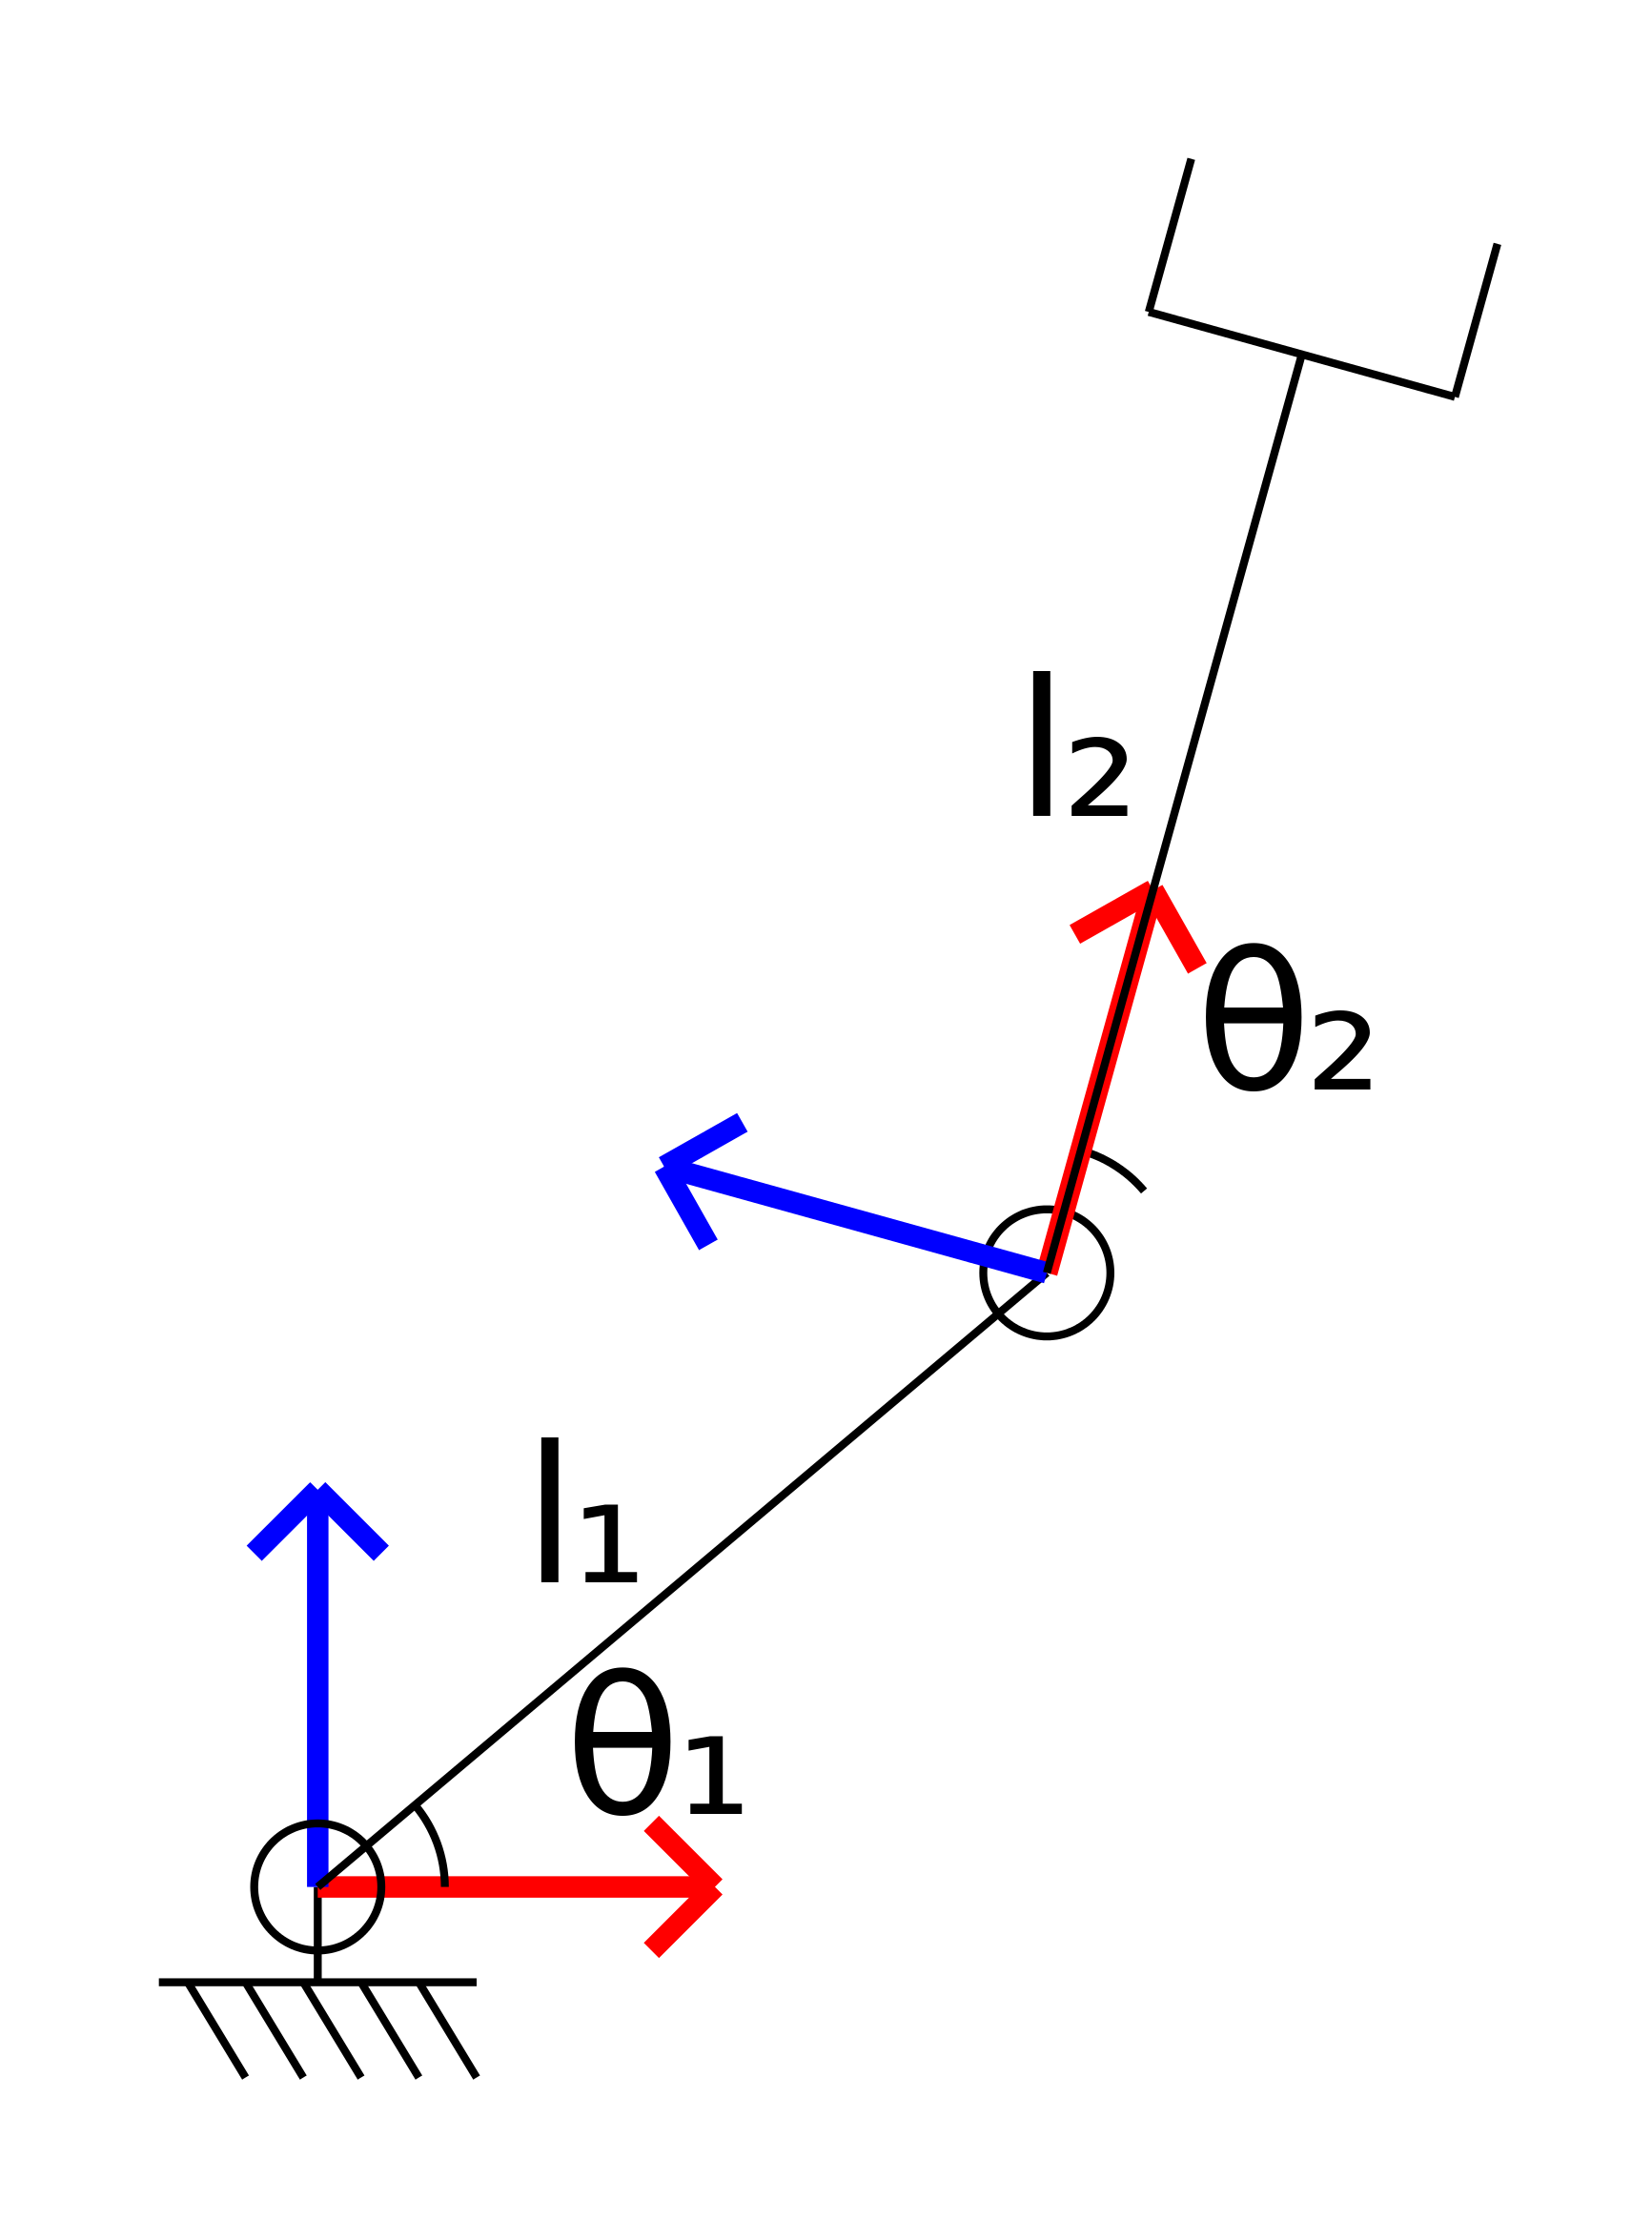
\includegraphics[scale=0.07]{generated_figures/RR_nonsingular.png}
    \end{center}
        Assume $\begin{bmatrix}
            \theta_1 \\
            \theta_2
        \end{bmatrix} = \begin{bmatrix}
            \frac\pi4 \\
            \frac\pi4
        \end{bmatrix}$.
        % \smcolvec{\th[1]\\\th[2]} =
        % \smcolvec{\piover{4}\\\piover{4}}.
    \begin{enumerate} [label=\alph*.]
        \item \text{[1 point]} What is the dimension of the end-effector Jacobian? Consider
        end effector positions $\begin{bmatrix} x \\ y \end{bmatrix} \in \mathbb{R}^2$.%\smcolvec{x\\y} in $\RR^2$.
        \begin{tcolorbox}[height=3cm]
            % TODO: ENTER YOUR ANSWER HERE
        \end{tcolorbox}
        
        \item \text{[1 point]} Is this system underconstrained, overconstrained, or neither?
        Why?
        \begin{tcolorbox}[height=3cm]
            % TODO: ENTER YOUR ANSWER HERE
        \end{tcolorbox}
        
        \item \text{[4 points]} On separate plots, draw the velocity vector for the end effector
        caused by:
        \begin{enumerate} [label=(\roman*)]
          \item Joint 1 moving with unit velocity (joints 2 has zero velocity).
          \item Joint 2 moving with unit velocity (joints 1 has zero velocity).
        \end{enumerate}
        The direction of these vectors should be correct, and the relative
        magnitudes should be approximately correct, but do not worry about
        exact magnitudes.  You can complete this problem by inspection or by
        using properties of the Jacobian.
        \begin{tcolorbox}[height=3cm]
            % TODO: ENTER YOUR ANSWER HERE
        \end{tcolorbox}
        
        \item \text{[2 points]} What is the dimension of the space spanned by these vectors?
        Are the 1st and 2nd vectors linearly independent?
        \begin{tcolorbox}[height=3cm]
            % TODO: ENTER YOUR ANSWER HERE
        \end{tcolorbox}
        
        \item \text{[1 point]} What is the rank of $J$ for this configuration?
        \begin{tcolorbox}[height=3cm]
            % TODO: ENTER YOUR ANSWER HERE
        \end{tcolorbox}
        
        \item \text{[1 point]} When identifying the inverse differential kinematics for this
        problem, would you use the inverse, the left psuedoinverse, or the right
        psuedoinverse?
        \begin{tcolorbox}[height=3cm]
            % TODO: ENTER YOUR ANSWER HERE
        \end{tcolorbox}
        
    \end{enumerate}

    \titledquestion{RRR Robot}
    Consider the following robot
    \begin{center}
    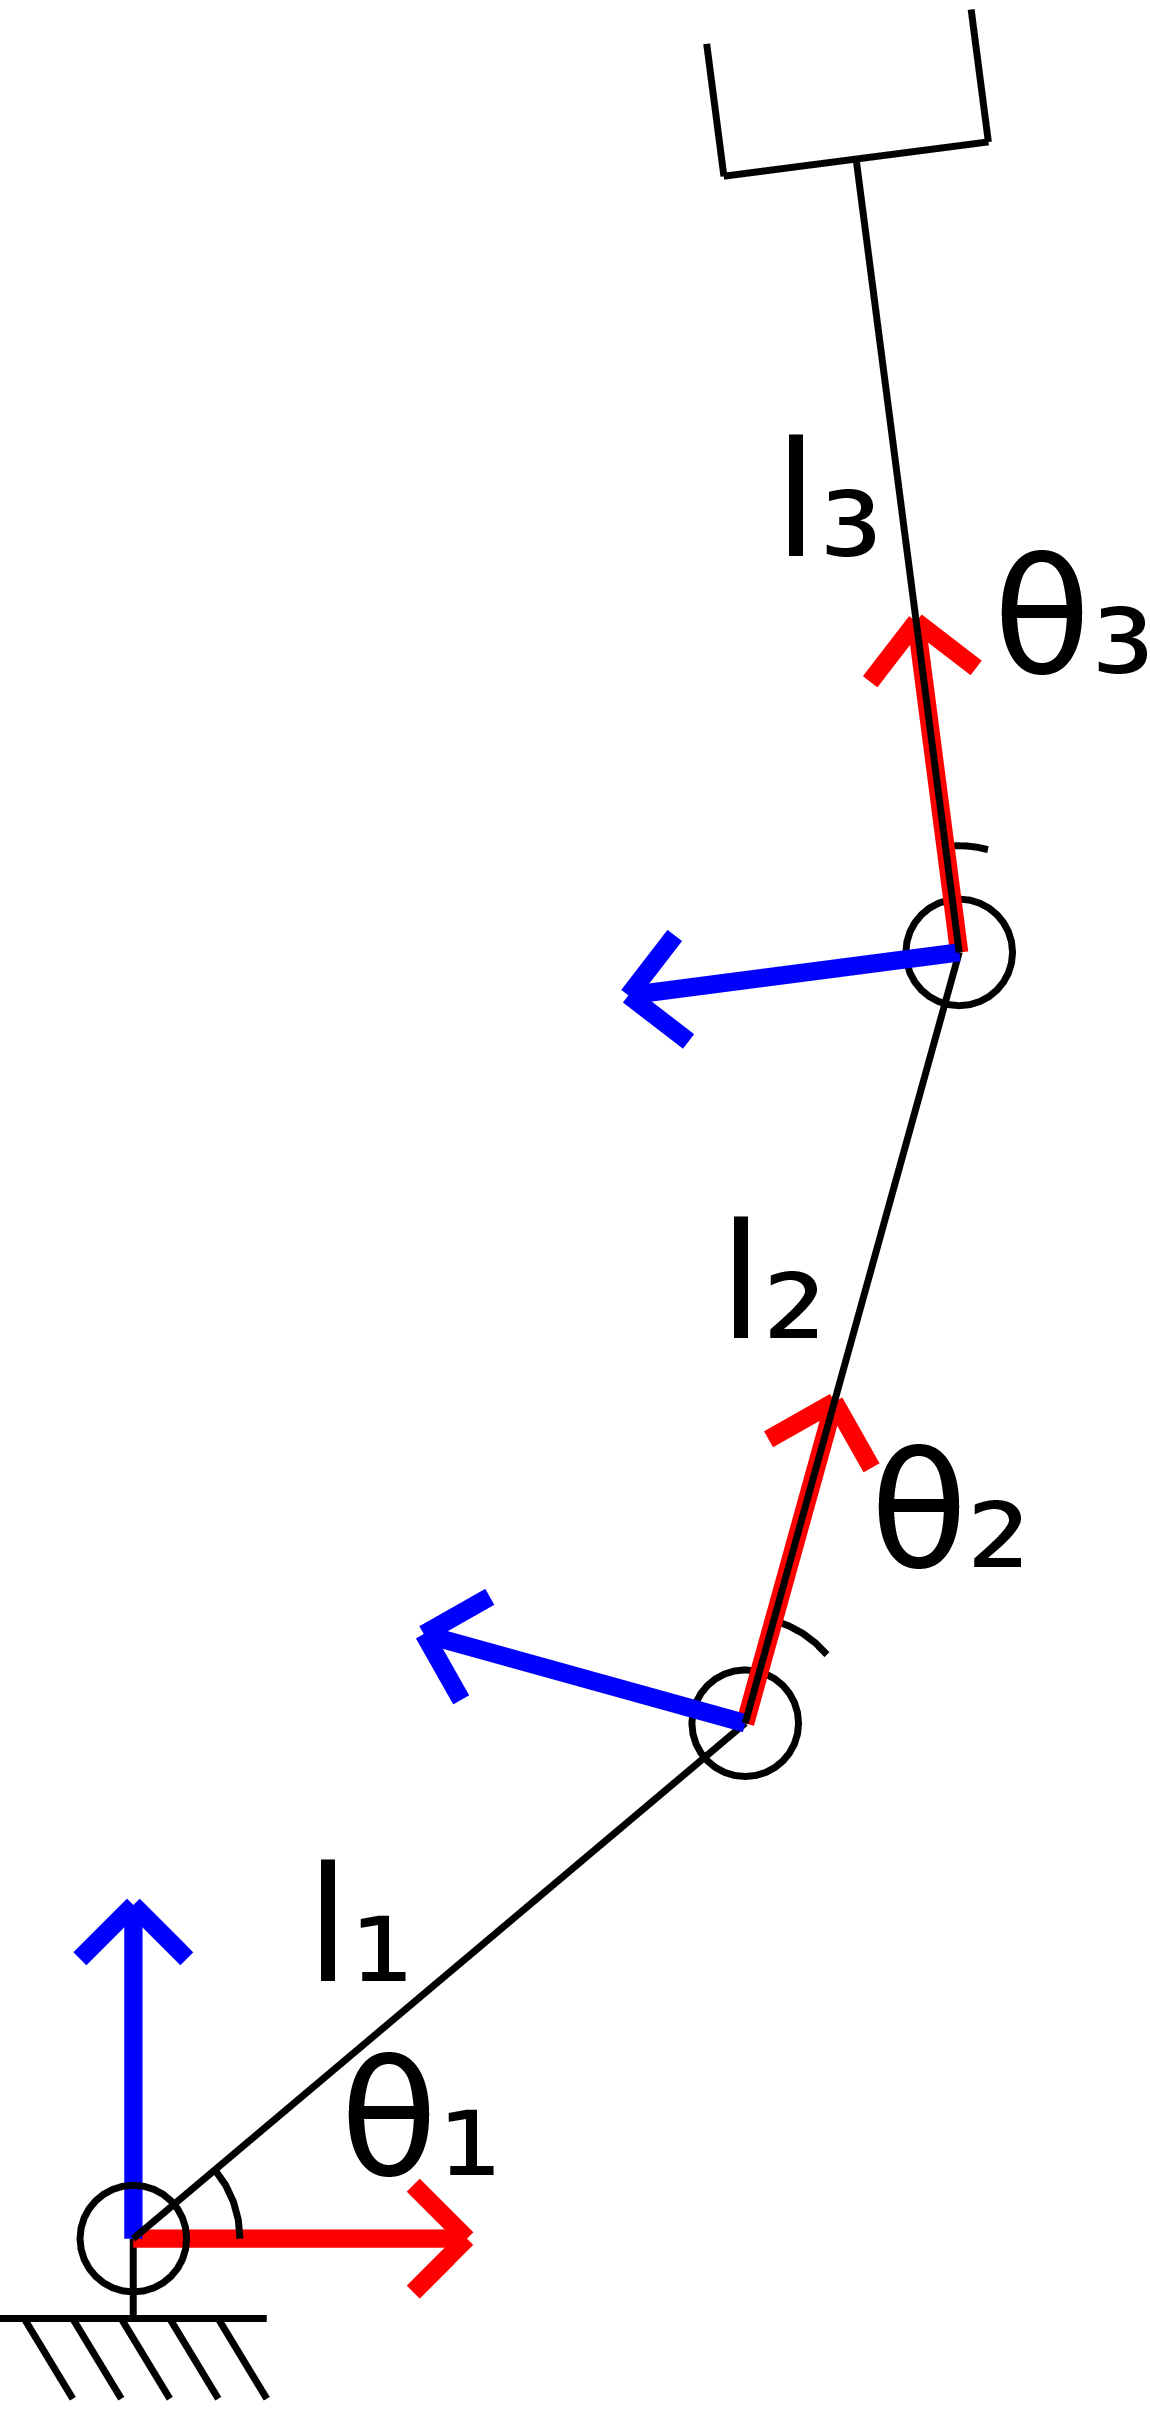
\includegraphics[scale=0.07]{generated_figures/RRR_nonsingular.png}
    \end{center}

    Assume $\begin{bmatrix}
        \theta_1 \\ \theta_2 \\ \theta_2
    \end{bmatrix} = \begin{bmatrix}
        \frac\pi3 \\ \frac\pi3 \\ \frac\pi3
    \end{bmatrix}$.
    % \smcolvec{\th[1]\\\th[2]\\\th[3]} =
    % \smcolvec{\piover{2}\\\piover{3}\\\piover{3}}.
    
     \begin{enumerate} [label=\alph*.]
        \item \text{[1 point]} What is the dimension of the end-effector Jacobian? Consider
        end effector positions $\begin{bmatrix}
            x \\ y
        \end{bmatrix} \in \mathbb{R}^2$. %\smcolvec{x\\y} in $\RR^2$.
        \begin{tcolorbox}[height=3cm]
            % TODO: ENTER YOUR ANSWER HERE
        \end{tcolorbox}
        
        \item \text{[1 point]} Is this system underconstrained, overconstrained, or neither?
        Why?
        \begin{tcolorbox}[height=3cm]
            % TODO: ENTER YOUR ANSWER HERE
        \end{tcolorbox}
        
        \item \text{[6 points]} On separate plots, draw the velocity vector for the end effector
        caused by
        \begin{enumerate} [label=(\roman*)]
          \item Joint 1 moving with unit velocity (joints 2 and 3 have zero velocity).
          \item Joint 2 moving with unit velocity (joints 1 and 3 have zero velocity).
          \item Joint 3 moving with unit velocity (joints 1 and 2 have zero velocity).
        \end{enumerate}
        The direction of these vectors should be correct, and the relative
        magnitudes should be approximately correct, but do not worry about
        exact magnitudes.  You can complete this problem by inspection or by
        using properties of the Jacobian.
        \begin{tcolorbox}[height=3cm]
            % TODO: ENTER YOUR ANSWER HERE
        \end{tcolorbox}
        
        \item \text{[2 points]} What is the dimension of the space spanned by these vectors?
        Are the 1st and 2nd vectors linearly independent? The 1st and 3rd?  The
        2nd and 3rd? All three?
        \begin{tcolorbox}[height=3cm]
            % TODO: ENTER YOUR ANSWER HERE
        \end{tcolorbox}
        
        \item \text{[1 point]} What is the rank of $J$ for this configuration?
        \begin{tcolorbox}[height=3cm]
            % TODO: ENTER YOUR ANSWER HERE
        \end{tcolorbox}
        
        \item \text{[1 point]} When identifying the inverse differential kinematics for this
        problem, would you use the inverse, the left psuedoinverse, or the right
        psuedoinverse?
        \begin{tcolorbox}[height=3cm]
            % TODO: ENTER YOUR ANSWER HERE
        \end{tcolorbox}
        
    \end{enumerate}

    \titledquestion{RRR Robot, revisited with rotation}

    Consider the following robot
    \begin{center}
    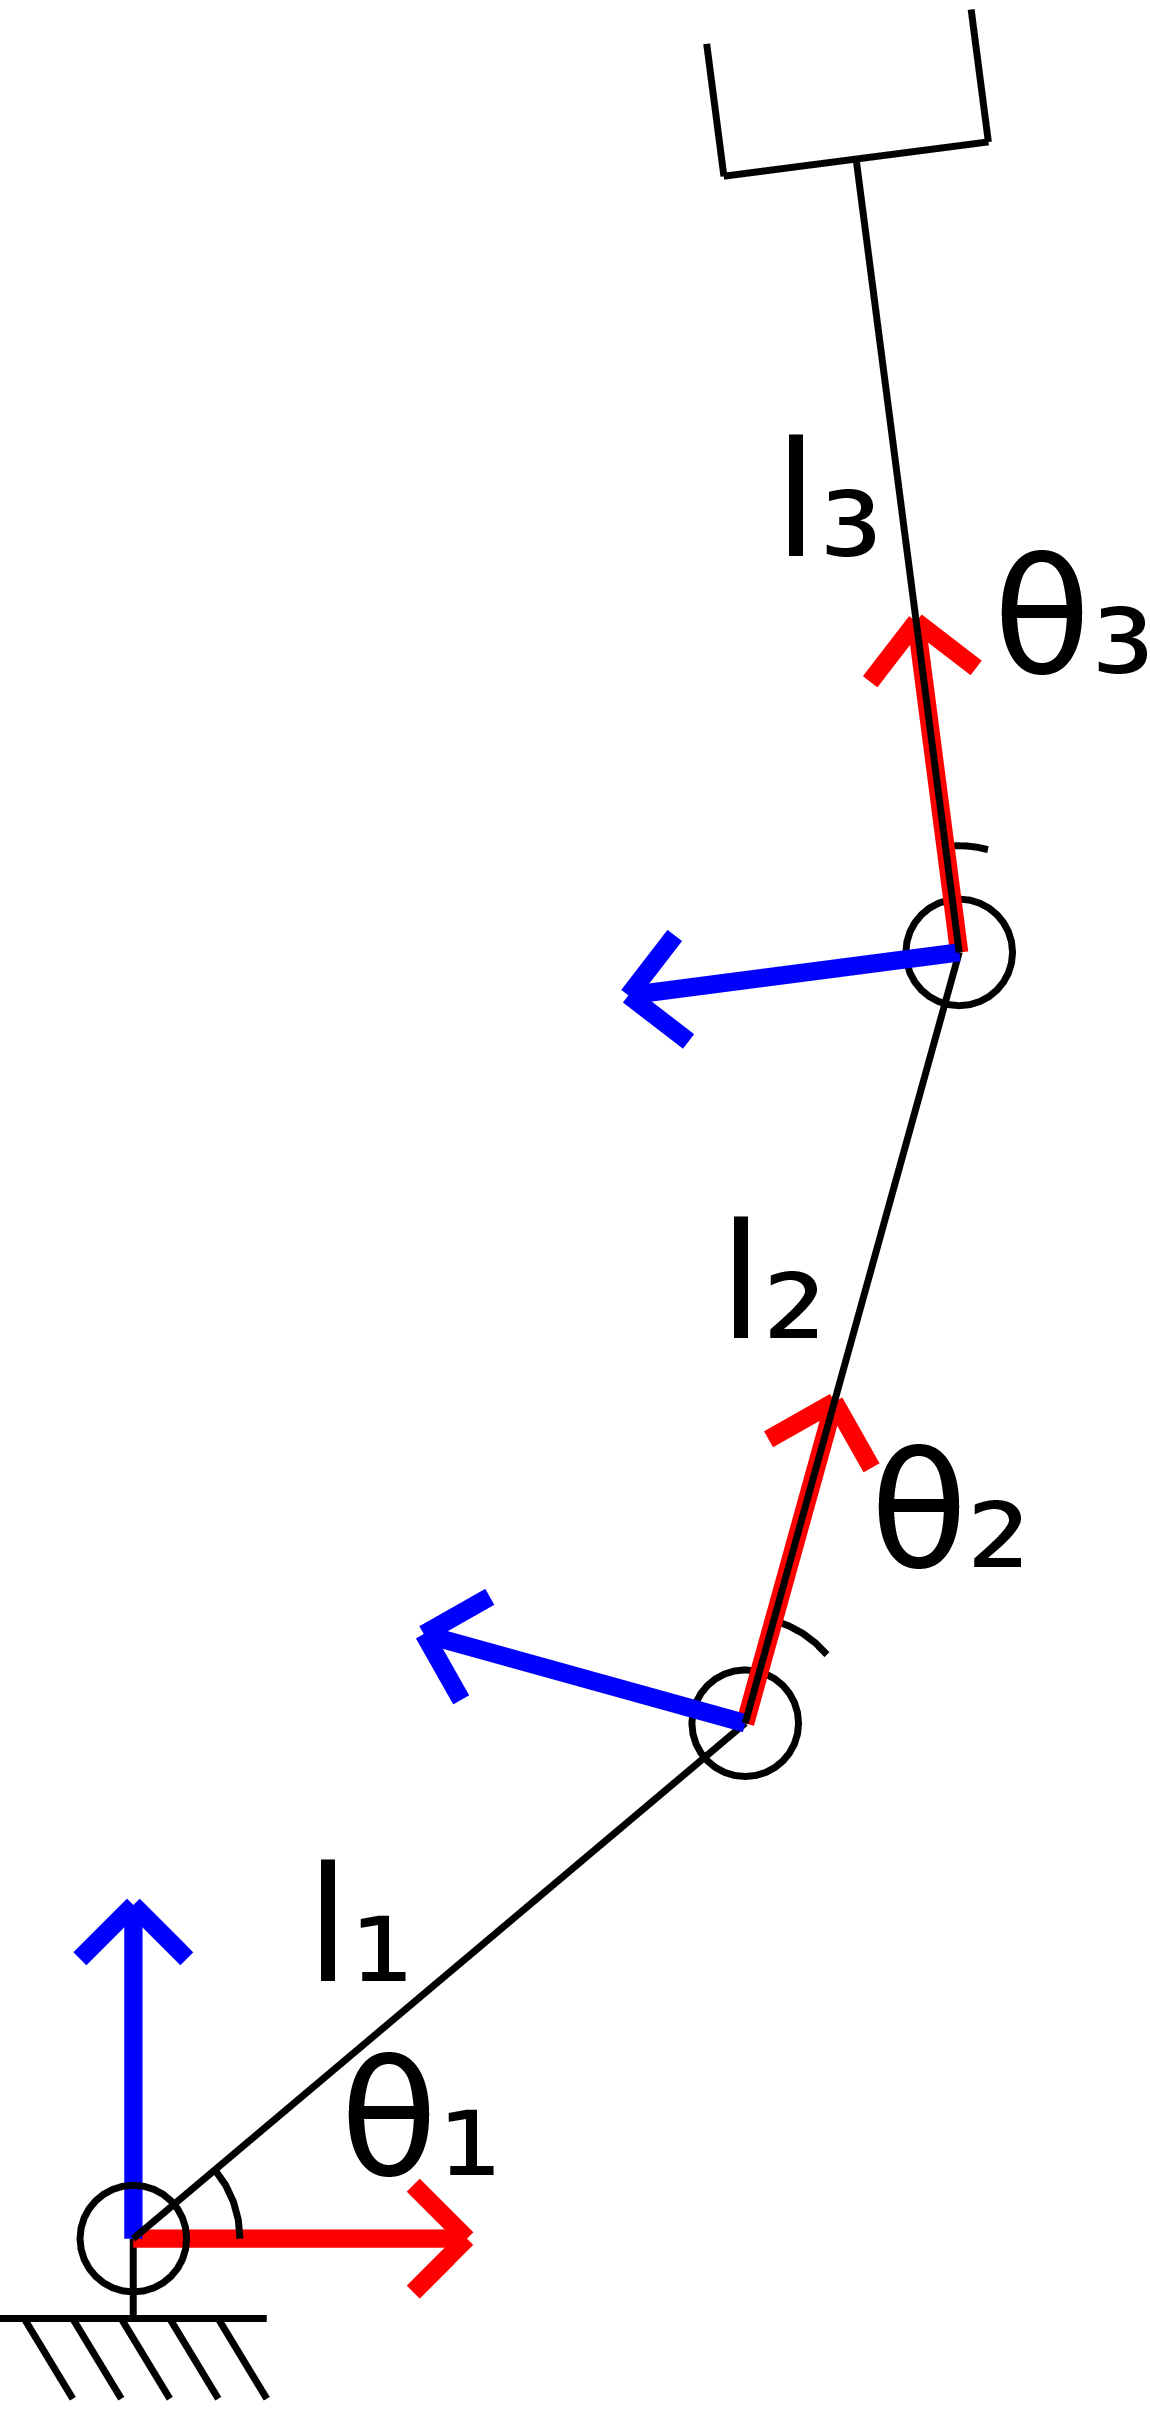
\includegraphics[scale=0.07]{generated_figures/RRR_nonsingular.png}
    \end{center}
    \begin{enumerate} [label=\alph*.]
        \item \text{[1 point]} What is the dimension of the end-effector Jacobian, now considering
        \begin{bmatrix}
            x \\ y \\ \theta
        \end{bmatrix}
        %\smcolvec{x\\y\\\th}
        end-effector positions in $SE(2)$.
        \begin{tcolorbox}[height=3cm]
            % TODO: ENTER YOUR ANSWER HERE
        \end{tcolorbox}
        
        \item \text{[1 point]} Is this system underconstrained, overconstrained, or neither?
        Why?
        \begin{tcolorbox}[height=3cm]
            % TODO: ENTER YOUR ANSWER HERE
        \end{tcolorbox}
        
        \item \text{[1 point]} Write out the end-effector Jacobian.
        \begin{tcolorbox}[height=3cm]
            % TODO: ENTER YOUR ANSWER HERE
        \end{tcolorbox}
        
        \item \text{[3 points]} Assume $\theta_1 = 0.6$, $\theta_2 = 0.6$, and $\theta_3 = 0.4$ (all
        values in radians). Write out the end-effector velocity $\begin{bmatrix} \dot x \\ \dot y \\ \dot z \end{bmatrix}$
        %\smcolvec{\xd\\\yd\\\thd} 
        for each of:
        \begin{enumerate} [label=(\roman*)]
          \item Joint 1 moving with unit velocity (joints 2 and 3 have zero velocity).
          \item Joint 2 moving with unit velocity (joints 1 and 3 have zero velocity).
          \item Joint 3 moving with unit velocity (joints 1 and 2 have zero velocity).
        \end{enumerate}
        \begin{tcolorbox}[height=3cm]
            % TODO: ENTER YOUR ANSWER HERE
        \end{tcolorbox}
        
        \item \text{[2 points]} What is the dimension of the space spanned by these vectors? Are
        the 1st and 2nd vectors linearly independent? The 1st and 3rd?  The 2nd
        and 3rd? All three?
        \begin{tcolorbox}[height=3cm]
            % TODO: ENTER YOUR ANSWER HERE
        \end{tcolorbox}
        
        \item \text{[1 point]} What is the rank of $J$ for this configuration?
        \begin{tcolorbox}[height=3cm]
            % TODO: ENTER YOUR ANSWER HERE
        \end{tcolorbox}
        
        \item \text{[2 points]} When identifying the inverse differential kinematics for this
        problem, would you use the inverse, the left psuedoinverse, or the right
        psuedoinverse?
        \begin{tcolorbox}[height=3cm]
            % TODO: ENTER YOUR ANSWER HERE
        \end{tcolorbox}
    \end{enumerate}

    \titledquestion{RRR Singular Configuration}

    Consider the following robot
    \begin{center}
    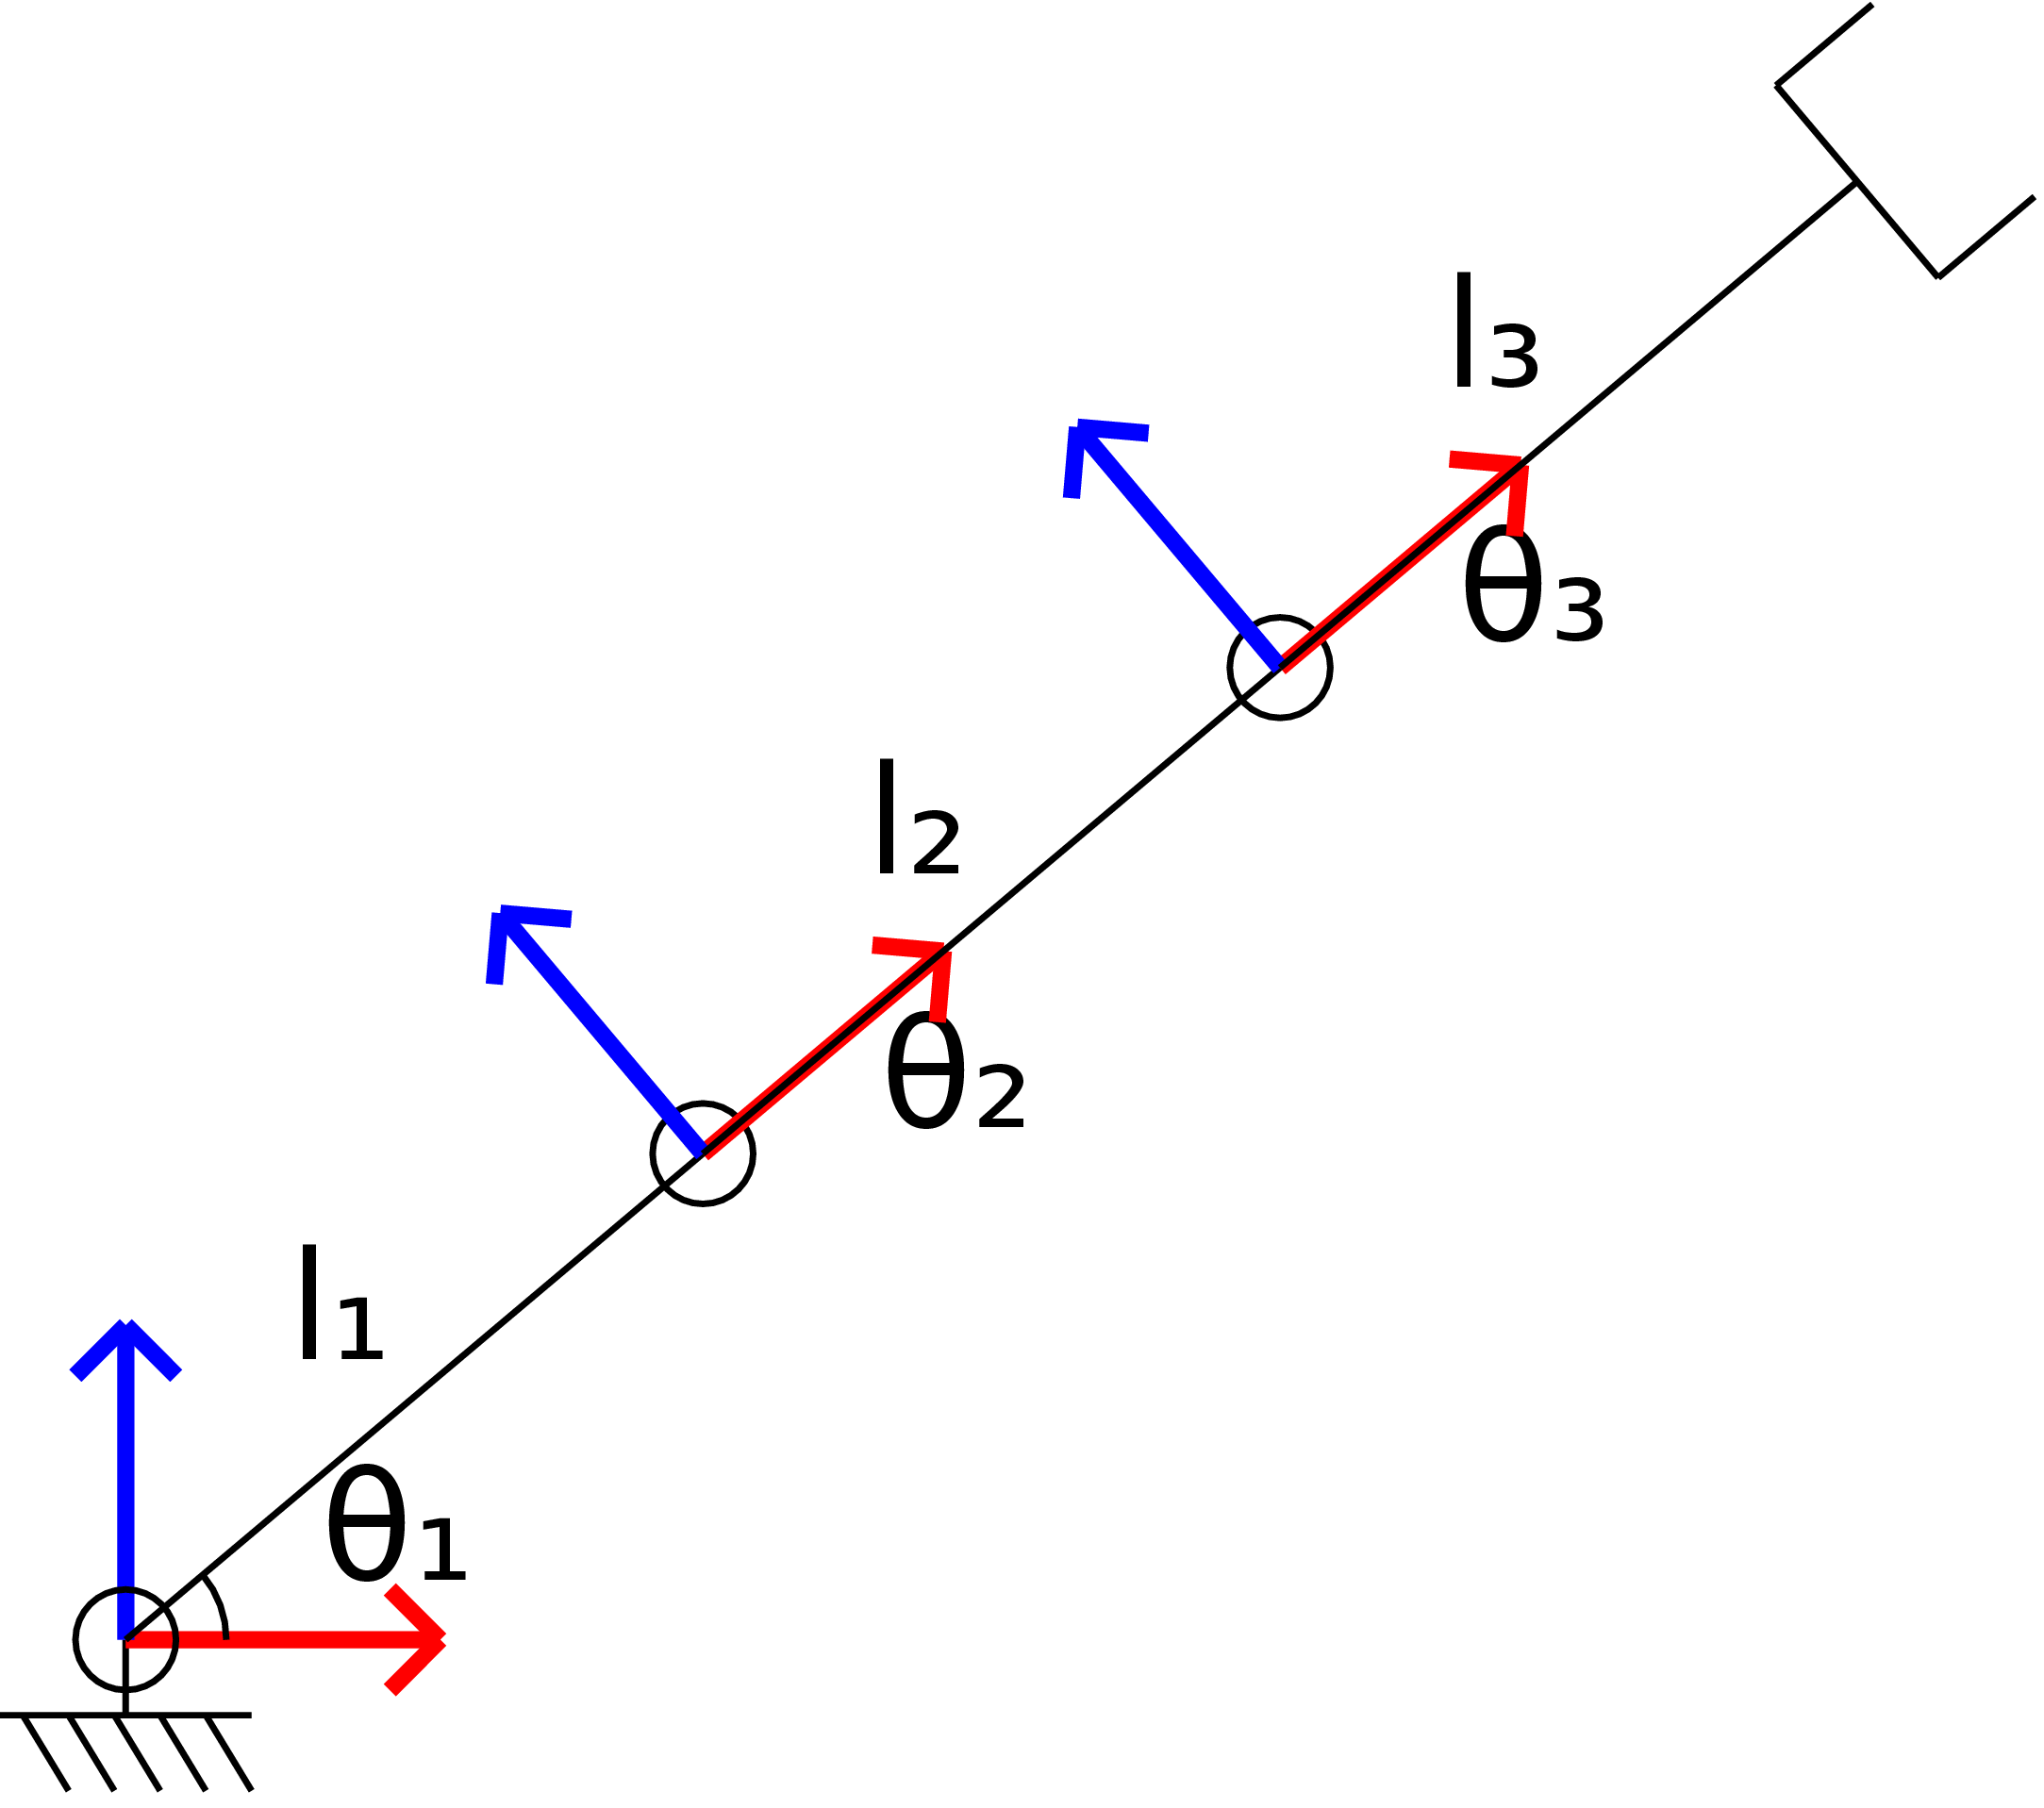
\includegraphics[scale=0.07]{generated_figures/RRR_singular.png}
    \end{center}
    \begin{enumerate} [label=\alph*.]
        \item \text{[1 point]} What is the dimension and rank of the end-effector Jacobian?
        Consider end effector positions $\begin{bmatrix} x \\ y \end{bmatrix} \in \mathbb{R}^2$.
        %\smcolvec{x\\y} in $\RR^2$.
        Do the dimension
        and rank differ? why?
        \begin{tcolorbox}[height=3cm]
            % TODO: ENTER YOUR ANSWER HERE
        \end{tcolorbox}
        
        \item \text{[6 points]} On separate plots, draw the velocity vector for the end effector
        caused by
        \begin{enumerate} [label=(\roman*)]
          \item Joint 1 moving with unit velocity (joints 2 and 3 have zero velocity).
          \item Joint 2 moving with unit velocity (joints 1 and 3 have zero velocity).
          \item Joint 3 moving with unit velocity (joints 1 and 2 have zero velocity).
        \end{enumerate}
        The direction of these vectors should be correct, and the relative
        magnitudes should be approximately correct, but do not worry about
        exact magnitudes.  You can complete this problem by inspection or by
        using properties of the Jacobian.
        \begin{tcolorbox}[height=3cm]
            % TODO: ENTER YOUR ANSWER HERE
        \end{tcolorbox}
        
        \item \text{[2 points]} What is the dimension of the space spanned by these vectors? Are
        the 1st and 2nd vectors linearly independent? The 1st and 3rd?  The 2nd
        and 3rd? All three?
        \begin{tcolorbox}[height=3cm]
            % TODO: ENTER YOUR ANSWER HERE
        \end{tcolorbox}
        
        \item \text{[1 point]} What is the rank of $J$ for this configuration?
        \begin{tcolorbox}[height=3cm]
            % TODO: ENTER YOUR ANSWER HERE
        \end{tcolorbox}
        
    \end{enumerate}

    \titledquestion{Local Inverse Kinematics}

    Consider a general arm with revolute joints. Assume you already have the
    kinematic map to the end effector, $f$, and the Jacobian of the end
    effector, $J$.

    The robot arm begins with joint angles $\Theta_0$, resulting in an
    end-effector position of $\mathbf{p}_0 = f(\Theta_0)$.  The end effector
    needs to pick up an object at point $\mathbf{p}_1$.

    Note: this is a conceptual problem: do not consider joint limits, and
    assume that all relevant positions are within the workspace of the robot.
    Furthermore, all answers are in terms of the given variables and known
    constants.
    
    \begin{enumerate} [label=\alph*.]
        \item \text{[2 points]} What are the initial joint angle velocities $\dot{\Theta}_0$ that
      start to move the end effector directly towards $\mathbf{p}_1$?
      \begin{tcolorbox}[height=3cm]
            % TODO: ENTER YOUR ANSWER HERE
        \end{tcolorbox}
        
        \item \text{[3 points]} Assume the end effector has moved at $\dot{\Theta}_0$ for a small
      amount of time $dt$.  What joint angles velocities $\dot{\Theta}_{dt}$
      will move the end effector from this new starting point directly towards
      $\mathbf{p}_1$?
      \begin{tcolorbox}[height=3cm]
            % TODO: ENTER YOUR ANSWER HERE
        \end{tcolorbox}
        
        \item \text{[2 points]} Describe (in a couple of sentences) how you would command the
      robot to move from $\mathbf{p}_0$ to $\mathbf{p}_1$ in approximately 1
      second.
      \begin{tcolorbox}[height=3cm]
            % TODO: ENTER YOUR ANSWER HERE
        \end{tcolorbox}
        
    \end{enumerate}

    Note that this process describes how differential IK can be used to solve
    IK \emph{numerically}, given a nearby starting point.  We will explore this
    concept in more depth in the next assignment.

\end{questions}


\section{Code Questions}
  
Copy the Code Handout folder to some location of your choice. Open Matlab and navigate to that location. Whenever you work on the assignment, go into this directory and run \verb!setup.m!. 

\begin{questions}
    \titledquestion{\text{[50 points]} General Robot Class} 
    Open directory \verb!ex_01!.
    Surely, you don't want to keep writing forward kinematics and Jacobians for
    every single assignment in this class!
    For this exercise, we will walk you through the creation of a general Python
    class that we will continue to use and extend for the remainder of this
    class. We will begin with writing forward kinematics for any RR arm, and
    then compute the Jacobian for any RR arm.
    First, open the file \verb!Robot.py!, and study this file. This is a basic Python
    class. The idea here is that you can pass parameters to the \emph{constructor} of
    the robot class, and the returned object then has methods that can be
    called, and can operate on the values you passed in. For example, the
    following code:
    \begin{verbatim}
    robot = Robot(np.array([[0.55], [0.4]]),\
    np.array([[1], [1]]), np.array([[1], [1]]), 0)

    
    frames = robot.fk(np.array([[0], [np.pi/2]]))
    \end{verbatim}
    can be used to find the forward kinematics of a robot with link lengths of
    0.55 and 0.4 for $\theta = \begin{bmatrix} 0 \\ \frac\pi2 \end{bmatrix}$
    \begin{center}
    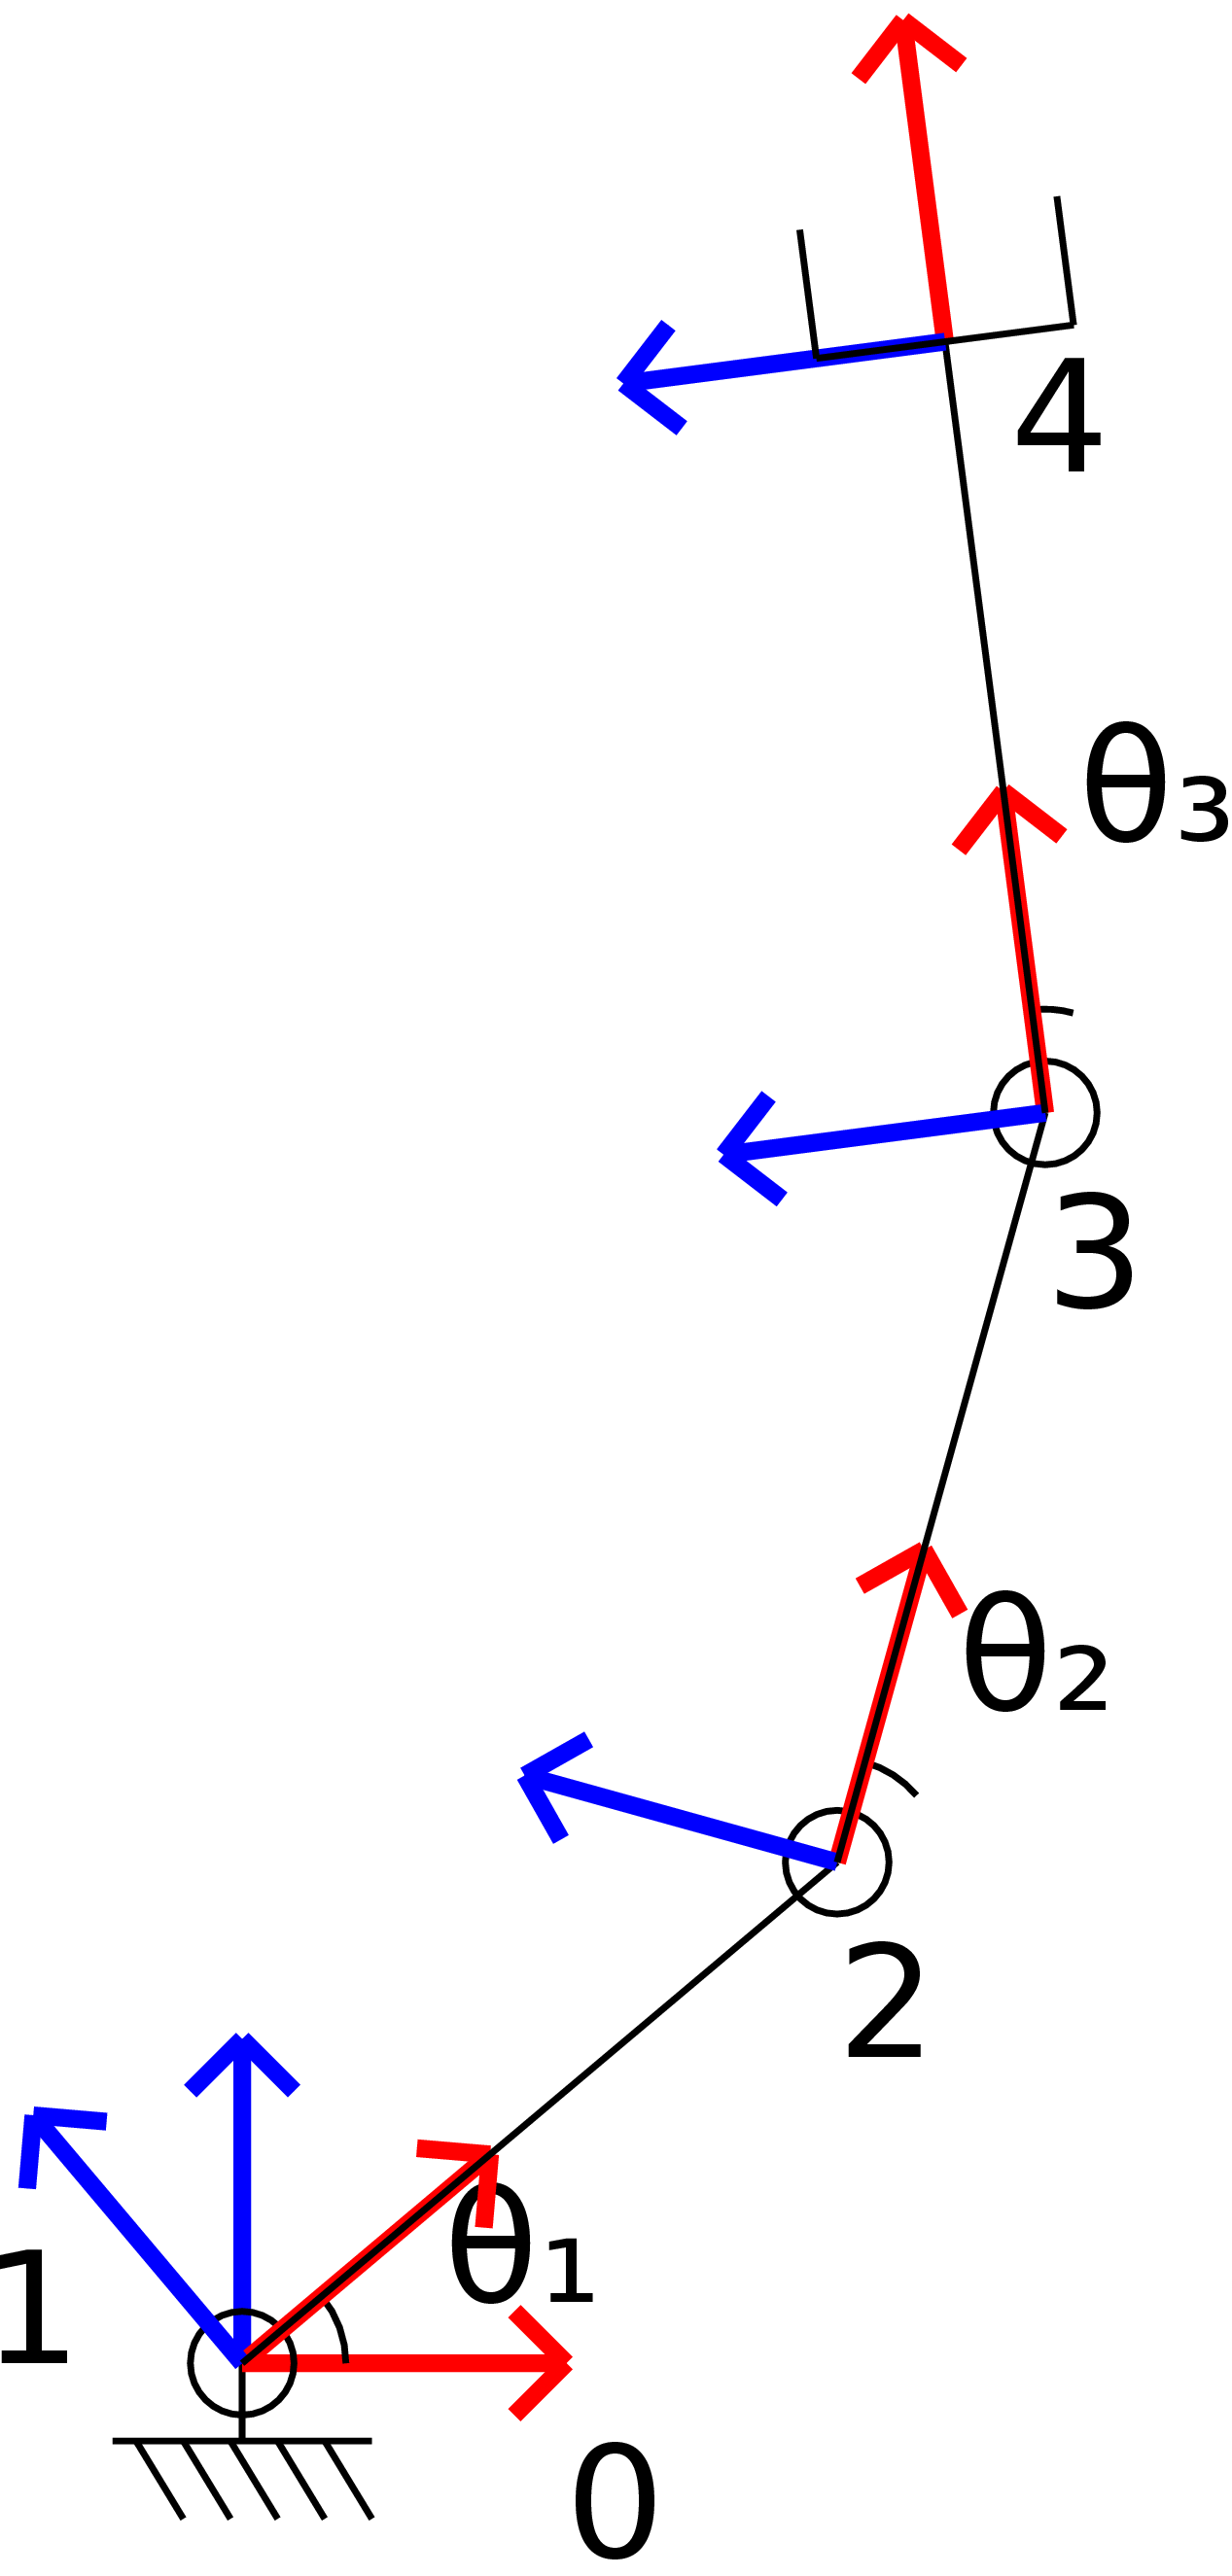
\includegraphics[scale=0.07]{generated_figures/RRR_alltheframes.png}
    \end{center}
    \paragraph{Forward Kinematics} Your job is to write forward kinematics that
    can work for any number of revolute joints in a chain. You will fill in
    the \verb!forward_kinematics! method in the \verb!Robot! class. This computes
    $H_i^0$ for each frame ($i > 0$) in the figure above, including the end
    effector frame.
    The code describes the conventions used for the resulting variable.
    One suggestion that should help is to break this problem into three
    components:
    \begin{itemize}
      \item First consider frame 1.
      \item Use a for loop to iterate from frame 2 to $n-1$; use 
      $H_{i-1}^0$ to help compute frame $H_i^0$.
      \item Compute the end effector frame, using $H_{n-1}^0$ to help.
    \end{itemize}
    \paragraph{Verification and Submission} To verify your results:
    \begin{enumerate}
      \item Run the \verb!sample_path! function. This will generate a plot and save
            two NumPy array files: \verb!calculated_path.npy! and \verb!ground_truth_path.npy!.
      \item The autograder on Gradescope will use a \verb!test_path_overlap.py! script to
            test your implementation. This script will load the saved paths, calculate
            the overlap between your calculated path and the ground truth, and verify
            that the overlap is 90\% or greater.
      \item To submit your work:
        \begin{itemize}
          \item Run the \verb!create_submission.py! script provided in the \verb!ex_01! directory.
                This will zip up all necessary files in the \verb!ex_01! folder.
          \item Submit the resulting zip file to Gradescope.
        \end{itemize}
    \end{enumerate}
    Save your sample path plot as a PNG and include it in your writeup. Also include
    an explanation of your forward kinematics implementation and any challenges you
    encountered.
\end{questions}

\begin{submissionChecklist}
			\item Create a PDF of your answers to the written questions with the name \verb!writeup.pdf!.
		\item Make sure you have \verb!writeup.pdf! in the same folder as the \verb!create_submission.m! script.
		\item Run \verb!create_submission.m! in Matlab.
		\item Upload \verb!handin-3.tar.gz! to Gradescope.
		\item Upload \verb!writeup.pdf! to Gradescope.
		% \item After completing the entire assignment, fill out the feedback
		% form\footnotemark.
		%~and make sure to add the submission code as the answer to the feedback section. 
		% \footnotetext{\texttt{\href{\feedbackURL}{\feedbackURL}}}
	\end{submissionChecklist}

\end{document}
